\chapter{Glycolysis: Taking Glucose Apart Step by Step}

\begin{kaichang}
Our old friend bread is back. In Chapter 46, we took apart its starch, a large molecule made from a long chain of glucose units holding hands. This time, look at something else: all those holes, large and small.

Leave freshly mixed dough somewhere warm, and after an hour or two it doubles in size. Press it, and it springs back softly; tear it open, and it is honeycombed inside. Baking sets those holes in place. Who inflated them? You know the answer: yeast. Yet yeast is a single-celled fungus less than a tenth of a hair's width across. It has no mouth, teeth, lungs, or bicycle pump. Simply sitting in dough, it turns sugar into gas, along with a little alcohol. Do not worry: almost all of that evaporates during baking.

Write down your guess: what happens inside a yeast cell that lets it eat sugar while blowing bubbles? Is the sugar burning inside? If so, why is the dough neither scalding hot nor aflame? We will return to your answer at the end of the chapter.
\end{kaichang}

\section{Invisible Activity in the Dough}

First, lay out what we can observe.

Disperse a little yeast in warm water and add a spoonful of sugar. Soon, foam appears on the surface, with a faint alcoholic, sour smell; the container wall feels slightly warm. At least three things are happening: \textbf{gas is being produced}, shown by foam; \textbf{new substances are forming}, shown by the alcoholic and sour smells; and \textbf{energy is escaping as heat}, shown by warming. Testing the gas with clear limewater makes it cloudy: the gas is carbon dioxide, the same molecule you breathe out, discussed in Chapter 32.

Consider some other familiar scenes. Milk left long enough becomes yogurt, whose sourness comes from lactic acid. After strenuous exercise, you gasp for breath and your muscles feel sore and heavy. A pickling jar, a wine vat, a steamer of buns: behind these seemingly unrelated things stand the same groups of microorganisms doing the same business, \textbf{extracting energy from sugar where oxygen is absent or insufficient}.

Now zoom into a yeast cell. Oxygen cannot enter or is insufficient, but the cell still has bills to pay: synthesizing materials, maintaining concentration differences across its membrane as in Chapter 51, and repairing parts. Where does the money come from? The cell has no furnace and cannot light a fire: its protein components would fall apart at flame temperatures through the denaturation discussed in Chapter 48. Its only capital is Chapter 46's glucose molecule, a six-carbon ring covered in hydroxyl groups.

What happens next is this chapter's subject: \textbf{glycolysis}. ``Glyco'' refers to sugar, here glucose, and ``lysis'' means breaking apart. As the name suggests, this reaction assembly line splits one six-carbon sugar into two three-carbon fragments.

\section{A Ten-Step Relay: Invest Before You Collect}

Glycolysis consists of ten reactions performed in relay by ten enzymes, whose abilities we explored in Chapter 49. All occur in the cytoplasm, without oxygen or any organelles. Even red blood cells, which lack mitochondria, and bacteria, far older than yeast, can do this. It is Earth's most widespread metabolic pathway: from bacteria to you, the ten steps are almost identical.

You need not memorize all ten steps, but you must understand the business logic of the two phases:

\begin{itemize}[itemsep=2pt]
\item \textbf{Investment phase, the first five steps:} the cell \textbf{pays out} two ATP molecules first. ATP attaches phosphate groups to glucose; Chapter 50 explained how phosphate transfer changes reactivity. Glucose is gradually reshaped into a form easy to split down the middle, then snaps into two small three-carbon molecules. It is like putting up capital to start a business.
\item \textbf{Payoff phase, the last five steps:} each three-carbon molecule undergoes several further modifications, losing parts and returning small payments. The energy released at each step is immediately used to make ATP, while electrons stripped from the carbon skeleton pass to the carrier \chem{NAD^{+}}, producing NADH. Each three-carbon molecule ultimately becomes a three-carbon pyruvic-acid molecule.
\end{itemize}

The balance sheet reads: 2 ATP invested, 4 produced, for a \textbf{net gain of 2 ATP}. There are also 2 NADH carrying high-energy electrons stripped from glucose, plus two pyruvic-acid molecules holding most of the carbon skeleton that remains to be dismantled.

\begin{center}
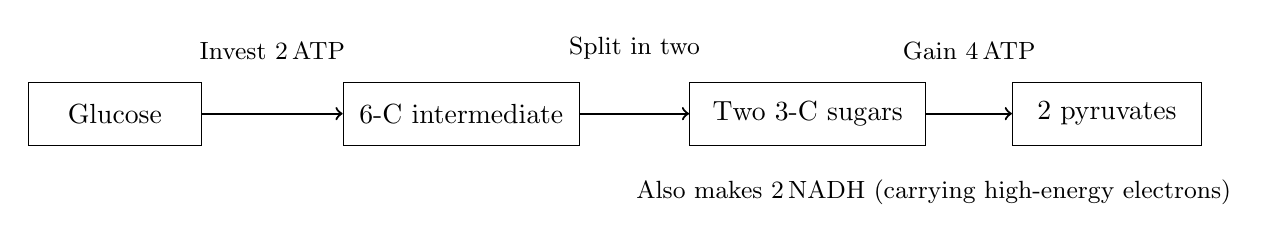
\begin{tikzpicture}[scale=1.0]
\node[draw,rectangle,minimum width=2.2cm,minimum height=0.8cm] (a) at (0,0) {Glucose};
\node[draw,rectangle,minimum width=3.0cm,minimum height=0.8cm] (b) at (4.4,0) {6-C intermediate};
\node[draw,rectangle,minimum width=3.0cm,minimum height=0.8cm] (c) at (8.8,0) {Two 3-C sugars};
\node[draw,rectangle,minimum width=2.4cm,minimum height=0.8cm] (d) at (12.6,0) {2 pyruvates};
\draw[->,thick] (a) -- (b) node[midway,above=16pt]{\small Invest $2\,\mathrm{ATP}$};
\draw[->,thick] (b) -- (c) node[midway,above=16pt]{\small Split in two};
\draw[->,thick] (c) -- (d) node[midway,above=16pt]{\small Gain $4\,\mathrm{ATP}$};
\node at (10.4,-1.0) {\small Also makes $2\,\mathrm{NADH}$ (carrying high-energy electrons)};
\end{tikzpicture}
\end{center}

This diagram is a human representation. Its boxes and arrows record substances and money coming and going, not actual molecular shapes. The real ten steps are much more detailed.

\section{Four Key Stations on the Assembly Line}

You need not learn the reactions' names, but four stations deserve a closer look because each answers a real question.

\textbf{First: what keeps glucose inside the cell?} After entering down its concentration gradient, glucose could in principle leave by the same route. The first enzyme solves this by stamping it: a phosphate group is taken from ATP and attached to glucose's carbon number 6. Phosphorylated glucose carries a negative charge, and membrane channels that recognize only neutral molecules no longer recognize it. The packaging changes as soon as the shipment enters the warehouse, preventing returns. The first ATP invested buys \textbf{exclusive access to the raw material}.

\textbf{Second: where should the six-carbon skeleton be cut?} Go straight to the investment phase's costliest cut: station three adds another phosphate group, reshaping the molecule into a bisphosphate chain held at both ends. The next enzyme cuts it right through the middle into two three-carbon sugars. Stretch first, then snip. The investment is not wasted: it positions the molecule so that it splits readily.

\textbf{Third: where are electrons removed?} The first payoff step is the pathway's only oxidation reaction; Chapter 28 defined oxidation as losing electrons. An enzyme oxidizes an aldehyde group on the three-carbon skeleton. The removed electrons, together with a proton, are accepted by waiting \chem{NAD^{+}}, producing NADH. A substantial part of glucose's stored energy resides in this extracted electron pair. \textbf{NADH is this chapter's real high-yield deposit}, although it cannot be cashed until Chapter 53.

\textbf{Fourth: where is ATP made?} At two payoff steps, a phosphate group on an intermediate is transferred directly to ADP, making ATP on the spot. Neither oxygen nor mitochondria are involved. Passing phosphate from a substrate molecule to ADP is called \textbf{substrate-level phosphorylation}. It produces ATP quickly but in limited quantities: just 4 direct transfers per glucose. Most of the human body's ATP actually comes from a more spectacular process, the subject of the next chapter.

\section{Who Applies the Brakes?}

Now for an easily overlooked question from the outline, but one close to the heart of life: how is this assembly line controlled?

A cell cannot dismantle sugar at full speed forever. Sugar is valuable; burning it furiously when ATP is already plentiful is like filling a pool that is already full. Control does not require the cell to make a decision. It uses chemical feedback written into molecules. The enzyme at station three, which adds the second phosphate group, happens to be the line's slowest and most irreversible gate. Its allosteric sites, the remote switches outside the active site introduced in Chapter 49, directly sense cellular energy status. High ATP means there is enough money, so ATP binds and \textbf{switches the enzyme off}. Conversely, accumulation of AMP, a product left after ATP is spent, signals an empty account; AMP binds and \textbf{switches it back on}. Listening to both income and IOUs, this gate enzyme automatically adjusts the whole line to the energy balance.

This is a practical example of the fourth recurring question, ``How is change controlled?'' Control requires no commander, only differences in an enzyme's affinity for small molecules. How hormones add a body-wide layer of control during feeding, fasting, and exercise---the story of insulin and glucagon---will unfold in Chapter 55.

\section{Why Not Burn It All at Once?}

You may wonder: all this effort, ten steps, and a net gain of only 2 ATP? Would burning glucose directly with oxygen not release far more energy?

It certainly would, but that abundance is precisely the problem. Recall Chapter 27: energy release is one issue; \textbf{the rate and form of its release} are another. On paper, glucose reacting with oxygen releases enormous energy. Yet once it happens, it is combustion: energy pours out as heat within a millionth of a second. For a cell, it would be like receiving a year's salary as burning banknotes. A considerable sum, but not a penny you can spend.

A cell's needs are specific. Each purchase---a muscle contraction, pumping a batch of ions, synthesizing part of a protein---requires a small payment on the order of tens of ATP, as Chapter 50 explained. The clever strategy is therefore not to release the most energy, but to \textbf{divide a large amount into small portions, each captured by another molecule the instant it is released}. Glycolysis's ten steps are ten little stairs. Each releases a little free energy, and a dedicated enzyme stands at each step, transferring it into ATP or NADH. Fire burns money for warmth; enzymes count it out on the spot.

\begin{qiaoliang}
We can quantify this account. Experiments show that complete combustion of 1 mole of glucose, \ud{180}{g}, in oxygen to carbon dioxide and water has a free-energy change of about \ud{-2870}{kJ/mol}. Under cellular conditions, hydrolysis of 1 mole of ATP releases about \ud{30}{kJ} of usable energy.

Per mole of glucose, glycolysis stores a net 2 moles of ATP, about \ud{60}{kJ}, just roughly two percent of 2870! Where does the rest go? It does not disappear; conservation of energy is serious business. Most remains locked in the chemical bonds of two pyruvic-acid and two NADH molecules, while a small amount escapes as heat, one reason dough warms.

In other words, glycolysis is not a complete withdrawal. It merely \textbf{snips off two small amounts} from glucose's large banknote for immediate needs. How is the whole note exchanged? Chapter 53 will explain. Consider the scale of these small payments again: the total mass of ATP your cells synthesize and consume daily is roughly your body weight. Each ATP molecule is spent and earned again several times per minute on average. Without this sugar-dismantling relay, you could not afford the energy to finish reading this sentence.
\end{qiaoliang}

\section{Symbols: Ten Steps in One Line}

Only now do we bring in symbols. Omitting every intermediate, glycolysis's balance sheet is:

\[\chem{C_6H_{12}O_6} + \chem{2ADP} + \chem{2P_{i}} + \chem{2NAD^{+}} \rightarrow \chem{2C_3H_4O_3} + \chem{2ATP} + \chem{2NADH} + \chem{2H^{+}} + \chem{2H_2O}\]

Read from left to right: one glucose molecule, \chem{C_6H_{12}O_6}, consumes two ADP, two phosphates, \chem{P_{i}}, meaning free inorganic phosphate, and two \chem{NAD^{+}}. It produces two pyruvic-acid molecules, \chem{C_3H_4O_3}, two ATP, and two NADH. Pay special attention to \chem{NAD^{+}}: it is a reactant. That means \textbf{the entire assembly line stops immediately if the cell runs out of \chem{NAD^{+}}}. Remember this: it unlocks the second half of the chapter.

\section{The \chem{NAD^{+}} Crisis: Fermentation to the Rescue}

An overlooked question now takes center stage. Each round of glycolysis consumes one \chem{NAD^{+}} molecule---actually two---to accept electrons. The cell's supply is tiny: if all of it were turned into capital letters, it would fill only a few lines. Think of it as the change in a cash-register drawer, which can run out within minutes. Without \chem{NAD^{+}}, glycolysis jams halfway through, ATP production stops, and the cell faces bankruptcy within minutes.

In cells with oxygen and mitochondria, NADH can courier its electrons to the mitochondria, unload them, and return to \chem{NAD^{+}} for reuse. Chapter 53 examines this delivery route. But yeast deep in dough, lactic-acid bacteria in yogurt vats, and vigorously contracting muscle cells whose oxygen supply cannot keep up face the same predicament: \textbf{the delivery route is closed or overloaded, NADH accumulates, and \chem{NAD^{+}} runs short}.

What can they do? These cells use a simple accounting trick: NADH hands its electrons to glycolysis's own products on the spot. This is \textbf{fermentation}. The two most common methods are:

\begin{itemize}[itemsep=2pt]
\item \textbf{Lactic-acid fermentation:} NADH transfers electrons directly to pyruvic acid, which becomes lactic acid. Your muscle cells do this during an oxygen-starved sprint; so do the bacteria that turn milk into yogurt and cabbage into pickles. The sourness is lactic acid's taste.
\item \textbf{Alcoholic fermentation:} yeast first removes one carbon from pyruvic acid, releasing it as a carbon-dioxide molecule---the origin of bread's holes! The remaining two-carbon fragment accepts NADH's electrons and becomes alcohol.
\end{itemize}

See the point? Lactic acid and alcohol \textbf{are not fermentation's purpose but its by-products}. The cell wants only to turn NADH back into \chem{NAD^{+}} so that glycolysis can keep producing its meager but lifesaving 2 ATP. Do not think of fermentation as a primitive version of anaerobic respiration. It is not an energy-producing pathway but an energy-producing pathway's \textbf{life-support system}. Lactic acid and alcohol are merely the cell's discarded electron waste. That waste happens to be appetizingly sour or intoxicatingly aromatic, so humans have built a business on it for millennia.

Another question often causes confusion: does lactic acid cause muscle soreness after exercise?

\begin{wuqu}
``Your muscles ache the day after exercise because lactic acid has accumulated.'' This claim is widespread, even among fitness trainers. But the counterevidence is clear. Measurements show that lactate in blood and muscles is mostly cleared \textbf{within an hour} after strenuous exercise stops, transported away for oxidation or conversion back to sugar. Next-day soreness arrives late and peaks one to two days after exercise, long after the lactate is gone. The more accepted explanation is microscopic muscle-fiber damage from unfamiliar exercise and the subsequent repair-related inflammation. Lactate is neither waste nor a toxin: the heart and other tissues can burn it directly as fuel. Sports-drink slogans about clearing lactic acid sell reassurance. Of course, unusually severe soreness or changes in urine color warrant medical attention, not a popular-science book.
\end{wuqu}

\section{Can Sugar Ferment Without Living Cells?}

\begin{zhengju}
By the mid-nineteenth century, brewing was a pillar of European industry, yet nobody understood fermentation. The French chemist Pasteur examined fermenting liquid under a microscope and always found living yeast multiplying. He also found that heating the liquid to kill yeast stopped fermentation. He declared fermentation a vital activity of living cells: without life, no fermentation.

The German chemist Liebig disagreed sharply. He thought fermentation was simply chemicals decomposing, with yeast present by coincidence. The argument lasted decades without resolution because it needed a decisive experiment: \textbf{kill and break up the yeast, then see whether the remaining juice still ferments sugar}. If it did, Pasteur's vital theory would fail; if not, Liebig would win.

The difficulty was technical: how could cells be thoroughly broken without destroying their chemicals? In 1897, the German chemist Eduard Buchner was working on something unrelated, using yeast extracts to study drug preservation. He ground yeast with fine sand, pressed out the juice, and added plenty of sucrose as a preservative. The juice began bubbling: sugar fermented in cell-free liquid, producing both alcohol and carbon dioxide. Realizing he had stumbled on something important, Buchner repeated the tests and published the conclusion: \textbf{fermentation does not require intact living cells; their chemicals are enough}.

The dispute ended with a twist. Liebig's chemical theory pointed in the right direction, but his simple decomposition did not exist. Pasteur's vital theory was wrong, yet his insistence on precise biological machinery was not wholly mistaken. The workers were an entire set of cellular enzymes, later called ``zymase''; the Greek roots of enzyme mean ``in yeast.'' Over the next forty-plus years, generations of biochemists, including Embden, Meyerhof, and Parnas, pieced together all ten steps by blocking particular reactions with inhibitors and isolating accumulated intermediates. The pathway is therefore also called the Embden--Meyerhof--Parnas pathway. Buchner received the 1907 Nobel Prize in Chemistry, but the true legacy was an idea: \textbf{life's activities can be reproduced, measured, and taken apart in a test tube}. The wall between biology and chemistry began falling with that cup of bubbling yeast juice.
\end{zhengju}

\begin{shiyan}
\textbf{Observe Yeast ``Breathing''} (safe to do at home)

Materials: a small packet of supermarket dry yeast, white sugar, warm water, two transparent plastic bottles, two balloons, and a marker.

Procedure: (1) Half-fill both bottles with warm water, about $35\,^{\circ}\mathrm{C}$, not hot to the touch. Add a spoonful of sugar to each and shake to dissolve. (2) Add half a packet of yeast to only one bottle and shake; leave the other without yeast as a control. (3) Fit and secure a balloon over each bottle opening. (4) Leave somewhere warm and observe every ten minutes for an hour.

Observations: does foam appear in the yeast bottle? Does its balloon gradually inflate? What happens in the control? After an hour, remove the balloons and gently waft the air from the bottle openings toward your nose. What do you smell?

Safety: use only food ingredients, never sealed glass containers. Continued gas production can make sealed glass bottles burst. Afterward, pour the liquid down the drain and wash the bottles and balloons. Do not drink the fermenting liquid: unwanted microbes may be present, and the enjoyment is in observing, not tasting.
\end{shiyan}

\section{When This Pathway Is Enough, and When It Is Not}

Every model has limits, and glycolysis is no exception. Its strengths are \textbf{speed} and \textbf{flexibility about location}. All ten enzymes are in the cytoplasm, ready to work without oxygen or organelles. During the first tens of seconds of a sprint, your muscles mainly rely on it. Mature red blood cells discard even their nuclei and mitochondria and live entirely on glycolysis. They only need enough ATP to transport oxygen; enough is enough.

Its weakness is equally clear: only 2 net ATP per glucose, an astonishingly low return on raw materials. Long-term reliance on it would be like burning furniture for warmth: warm enough, but soon the house is empty. That is why it must cooperate with two downstream pathways. With oxygen, pyruvic acid and NADH enter mitochondria for further processing in Chapter 53; without oxygen, fermentation disposes of electron waste to keep it running.

Medicine makes use of glycolysis's habits. Many cancer cells avidly consume glucose through glycolysis even when oxygen is plentiful, a phenomenon called the Warburg effect whose causes remain under study. Doctors inject a mildly radioactive glucose analog; the more a cancer cell takes up, the stronger its signal. PET scans thus light up tumors. The sugar from our opening becomes a scout. This \textbf{does not} mean that eating sugar feeds cancer or avoiding it cures cancer: blood glucose is tightly regulated, extreme sugar avoidance lacks supporting evidence, and specific dietary questions belong with your doctor.

\section{Back to the Dough}

Now check your original answer. Yeast did not burn sugar: it used a ten-step relay, first breaking glucose into pyruvic acid and earning 2 ATP. With oxygen scarce deep in the dough, alcoholic fermentation regenerates \chem{NAD^{+}}, discarding carbon dioxide and alcohol as electron waste. The gluten network traps carbon dioxide in little gas chambers, forming bread's holes. In an oven at around $200\,^{\circ}\mathrm{C}$, the alcohol almost entirely evaporates, leaving a hint of baked aroma. The warmth you feel is energy that ATP did not capture on those ten steps, escaping as heat.

The dough neither scalds nor flames because energy is never released all at once: enzymes divide it step by step and capture it portion by portion. The difference between flames and bread is not the amount of energy released but \textbf{its release rate and destination}. That principle, repeated since Chapter 27, holds inside cells too.

\section{Breaking Down Is Only the Beginning}

Looking back, we have done only half the job, taking glucose as far as pyruvic acid. Two pyruvic-acid molecules and two NADH still hold more than ninety percent of glucose's energy, and the cell will not let it go. Where oxygen is plentiful, pyruvic acid enters the mitochondrial power plant and is broken down until only carbon dioxide remains. NADH hands off electrons that descend a protein conveyor belt in stages, ultimately driving a rotating molecular motor that makes ATP in bulk. Waiting at the electrons' destination is an old friend: oxygen. Why must it wait there? How would the conveyor belt fail without it? Next chapter, we will visit mitochondria to find out.

\begin{tiaozhan}
If \chem{NAD^{+}} is so important, what lets it accept electrons? Its full name is nicotinamide adenine dinucleotide. A nicotinamide ring in the molecule can accept a pair of electrons and a proton to become NADH: essentially a redox half-reaction, in Chapter 28's language. The total cellular amount of \chem{NAD^{+}} plus NADH is approximately fixed, and their ratio is an electron inventory. Predominant NADH means plenty of fuel and a backlog of electrons, so the cell slows breakdown and turns toward synthesis. Predominant \chem{NAD^{+}} means empty stores and faster glycolysis. Glycolysis's third enzyme, phosphofructokinase, follows this inventory: abundant ATP directly inhibits it. Product and raw material share an origin, so producing more means stopping more. Chapter 55 shows how the metabolic network uses downstream products to control upstream valves, coordinating hundreds of pathways into a self-regulating machine. You can skip these details without losing the main argument, but remember: regulation is automatic feedback written into chemical affinity, not a cell deciding what to do.
\end{tiaozhan}

\section*{Practice}

\begin{sikaoti}
\item Draw a material-flow diagram starting with one glucose molecule: invest 2 ATP, split into two halves, gain 4 ATP and 2 NADH, and obtain 2 pyruvic-acid molecules. Use arrows to show ATP entering and leaving. Including the initial investment, what is glycolysis's return on investment?
\item A can of cola contains about \ud{35}{g} of sugar, roughly 0.2 moles. If all this glucose undergoes only glycolysis, how many net moles of ATP result? Compare with the text's 2870 kJ/mol from complete oxidation and explain why glycolysis alone, like burning furniture for warmth, is not sustainable.
\item If a yogurt vat is poorly sealed and air enters, the lactic-acid bacteria's fermentation efficiency falls, an aspect of the Pasteur effect. Use this chapter's logic of \chem{NAD^{+}} regeneration to explain why cells become less dependent on fermentation when oxygen arrives.
\item Why could Buchner's yeast-juice experiment resolve the dispute between the vital and chemical theories? If the juice had not fermented at all, which side would the conclusion have favored? What does this tell you about the requirements for a decisive experiment?
\item An advertisement claims: ``This drink contains L-lactic acid to rapidly neutralize exercise-generated lactic acid and eliminate fatigue.'' Identify at least two scientific errors and refute them using this chapter.
\item Mature red blood cells lack mitochondria and rely entirely on glycolysis. Given that their job is to transport oxygen, suggest an advantage of obtaining energy through glycolysis without consuming oxygen.
\end{sikaoti}
